
%% bare_conf.tex
%% V1.4b
%% 2015/08/26
%% by Michael Shell
%% See:
%% http://www.michaelshell.org/
%% for current contact information.
%%
%% This is a skeleton file demonstrating the use of IEEEtran.cls
%% (requires IEEEtran.cls version 1.8b or later) with an IEEE
%% conference paper.
%%
%% Support sites:
%% http://www.michaelshell.org/tex/ieeetran/
%% http://www.ctan.org/pkg/ieeetran
%% and
%% http://www.ieee.org/

%%*************************************************************************
%% Legal Notice:
%% This code is offered as-is without any warranty either expressed or
%% implied; without even the implied warranty of MERCHANTABILITY or
%% FITNESS FOR A PARTICULAR PURPOSE! 
%% User assumes all risk.
%% In no event shall the IEEE or any contributor to this code be liable for
%% any damages or losses, including, but not limited to, incidental,
%% consequential, or any other damages, resulting from the use or misuse
%% of any information contained here.
%%
%% All comments are the opinions of their respective authors and are not
%% necessarily endorsed by the IEEE.
%%
%% This work is distributed under the LaTeX Project Public License (LPPL)
%% ( http://www.latex-project.org/ ) version 1.3, and may be freely used,
%% distributed and modified. A copy of the LPPL, version 1.3, is included
%% in the base LaTeX documentation of all distributions of LaTeX released
%% 2003/12/01 or later.
%% Retain all contribution notices and credits.
%% ** Modified files should be clearly indicated as such, including  **
%% ** renaming them and changing author support contact information. **
%%*************************************************************************


% *** Authors should verify (and, if needed, correct) their LaTeX system  ***
% *** with the testflow diagnostic prior to trusting their LaTeX platform ***
% *** with production work. The IEEE's font choices and paper sizes can   ***
% *** trigger bugs that do not appear when using other class files.       ***                          ***
% The testflow support page is at:
% http://www.michaelshell.org/tex/testflow/



\documentclass[conference]{IEEEtran}
% Some Computer Society conferences also require the compsoc mode option,
% but others use the standard conference format.
%
% If IEEEtran.cls has not been installed into the LaTeX system files,
% manually specify the path to it like:
% \documentclass[conference]{../sty/IEEEtran}
\usepackage{graphicx}
\usepackage{cite}
\usepackage{url}
\usepackage{listings}
\usepackage{float,subcaption}
\usepackage{amsmath}
\usepackage{tikz}
\graphicspath{{images/}}
	




% Some very useful LaTeX packages include:
% (uncomment the ones you want to load)


% *** MISC UTILITY PACKAGES ***
%
%\usepackage{ifpdf}
% Heiko Oberdiek's ifpdf.sty is very useful if you need conditional
% compilation based on whether the output is pdf or dvi.
% usage:
% \ifpdf
%   % pdf code
% \else
%   % dvi code
% \fi
% The latest version of ifpdf.sty can be obtained from:
% http://www.ctan.org/pkg/ifpdf
% Also, note that IEEEtran.cls V1.7 and later provides a builtin
% \ifCLASSINFOpdf conditional that works the same way.
% When switching from latex to pdflatex and vice-versa, the compiler may
% have to be run twice to clear warning/error messages.






% *** CITATION PACKAGES ***
%
%\usepackage{cite}
% cite.sty was written by Donald Arseneau
% V1.6 and later of IEEEtran pre-defines the format of the cite.sty package
% \cite{} output to follow that of the IEEE. Loading the cite package will
% result in citation numbers being automatically sorted and properly
% "compressed/ranged". e.g., [1], [9], [2], [7], [5], [6] without using
% cite.sty will become [1], [2], [5]--[7], [9] using cite.sty. cite.sty's
% \cite will automatically add leading space, if needed. Use cite.sty's
% noadjust option (cite.sty V3.8 and later) if you want to turn this off
% such as if a citation ever needs to be enclosed in parenthesis.
% cite.sty is already installed on most LaTeX systems. Be sure and use
% version 5.0 (2009-03-20) and later if using hyperref.sty.
% The latest version can be obtained at:
% http://www.ctan.org/pkg/cite
% The documentation is contained in the cite.sty file itself.






% *** GRAPHICS RELATED PACKAGES ***
%
\ifCLASSINFOpdf
  % \usepackage[pdftex]{graphicx}
  % declare the path(s) where your graphic files are
  % \graphicspath{{../pdf/}{../jpeg/}}
  % and their extensions so you won't have to specify these with
  % every instance of \includegraphics
  % \DeclareGraphicsExtensions{.pdf,.jpeg,.png}
\else
  % or other class option (dvipsone, dvipdf, if not using dvips). graphicx
  % will default to the driver specified in the system graphics.cfg if no
  % driver is specified.
  % \usepackage[dvips]{graphicx}
  % declare the path(s) where your graphic files are
  % \graphicspath{{../eps/}}
  % and their extensions so you won't have to specify these with
  % every instance of \includegraphics
  % \DeclareGraphicsExtensions{.eps}
\fi
% graphicx was written by David Carlisle and Sebastian Rahtz. It is
% required if you want graphics, photos, etc. graphicx.sty is already
% installed on most LaTeX systems. The latest version and documentation
% can be obtained at: 
% http://www.ctan.org/pkg/graphicx
% Another good source of documentation is "Using Imported Graphics in
% LaTeX2e" by Keith Reckdahl which can be found at:
% http://www.ctan.org/pkg/epslatex
%
% latex, and pdflatex in dvi mode, support graphics in encapsulated
% postscript (.eps) format. pdflatex in pdf mode supports graphics
% in .pdf, .jpeg, .png and .mps (metapost) formats. Users should ensure
% that all non-photo figures use a vector format (.eps, .pdf, .mps) and
% not a bitmapped formats (.jpeg, .png). The IEEE frowns on bitmapped formats
% which can result in "jaggedy"/blurry rendering of lines and letters as
% well as large increases in file sizes.
%
% You can find documentation about the pdfTeX application at:
% http://www.tug.org/applications/pdftex





% *** MATH PACKAGES ***
%
%\usepackage{amsmath}
% A popular package from the American Mathematical Society that provides
% many useful and powerful commands for dealing with mathematics.
%
% Note that the amsmath package sets \interdisplaylinepenalty to 10000
% thus preventing page breaks from occurring within multiline equations. Use:
%\interdisplaylinepenalty=2500
% after loading amsmath to restore such page breaks as IEEEtran.cls normally
% does. amsmath.sty is already installed on most LaTeX systems. The latest
% version and documentation can be obtained at:
% http://www.ctan.org/pkg/amsmath





% *** SPECIALIZED LIST PACKAGES ***
%
%\usepackage{algorithmic}
% algorithmic.sty was written by Peter Williams and Rogerio Brito.
% This package provides an algorithmic environment fo describing algorithms.
% You can use the algorithmic environment in-text or within a figure
% environment to provide for a floating algorithm. Do NOT use the algorithm
% floating environment provided by algorithm.sty (by the same authors) or
% algorithm2e.sty (by Christophe Fiorio) as the IEEE does not use dedicated
% algorithm float types and packages that provide these will not provide
% correct IEEE style captions. The latest version and documentation of
% algorithmic.sty can be obtained at:
% http://www.ctan.org/pkg/algorithms
% Also of interest may be the (relatively newer and more customizable)
% algorithmicx.sty package by Szasz Janos:
% http://www.ctan.org/pkg/algorithmicx




% *** ALIGNMENT PACKAGES ***
%
%\usepackage{array}
% Frank Mittelbach's and David Carlisle's array.sty patches and improves
% the standard LaTeX2e array and tabular environments to provide better
% appearance and additional user controls. As the default LaTeX2e table
% generation code is lacking to the point of almost being broken with
% respect to the quality of the end results, all users are strongly
% advised to use an enhanced (at the very least that provided by array.sty)
% set of table tools. array.sty is already installed on most systems. The
% latest version and documentation can be obtained at:
% http://www.ctan.org/pkg/array


% IEEEtran contains the IEEEeqnarray family of commands that can be used to
% generate multiline equations as well as matrices, tables, etc., of high
% quality.




% *** SUBFIGURE PACKAGES ***
%\ifCLASSOPTIONcompsoc
%  \usepackage[caption=false,font=normalsize,labelfont=sf,textfont=sf]{subfig}
%\else
%  \usepackage[caption=false,font=footnotesize]{subfig}
%\fi
% subfig.sty, written by Steven Douglas Cochran, is the modern replacement
% for subfigure.sty, the latter of which is no longer maintained and is
% incompatible with some LaTeX packages including fixltx2e. However,
% subfig.sty requires and automat\usepackage{amsmath}ically loads Axel Sommerfeldt's caption.sty
% which will override IEEEtran.cls' handling of captions and this will result
% in non-IEEE style figure/table captions. To prevent this problem, be sure
% and invoke subfig.sty's "caption=false" package option (available since
% subfig.sty version 1.3, 2005/06/28) as this is will preserve IEEEtran.cls
% handling of captions.
% Note that the Computer Society format requires a larger sans serif font
% than the serif footnote size font used in traditional IEEE formatting
% and thus the need to invoke different subfig.sty package options depending
% on whether compsoc mode has been enabled.
%
% The latest version and documentation of subfig.sty can be obtained at:
% http://www.ctan.org/pkg/subfig




% *** FLOAT PACKAGES ***
%
%\usepackage{fixltx2e}
% fixltx2e, the successor to the earlier fix2col.sty, was written by
% Frank Mittelbach and David Carlisle. This package corrects a few problems
% in the LaTeX2e kernel, the most notable of which is that in current
% LaTeX2e releases, the ordering of single and double column floats is not
% guaranteed to be preserved. Thus, an unpatched LaTeX2e can allow a
% single column figure to be placed prior to an earlier double column
% figure.
% Be aware that LaTeX2e kernels dated 2015 and later have fixltx2e.sty's
% corrections already built into the system in which case a warning will
% be issued if an attempt is made to load fixltx2e.sty as it is no longer
% needed.
% The latest version and documentation can be found at:
% http://www.ctan.org/pkg/fixltx2e


%\usepackage{stfloats}
% stfloats.sty was written by Sigitas Tolusis. This package gives LaTeX2e
% the ability to do double column floats at the bottom of the page as well
% as the top. (e.g., "\begin{figure*}[!b]" is not normally possible in
% LaTeX2e). It also provides a command:
%\fnbelowfloat
% to enable the placement of footnotes below bottom floats (the standard
% LaTeX2e kernel puts them above bottom floats). This is an invasive package
% which rewrites many portions of the LaTeX2e float routines. It may not work
% with other packages that modify the LaTeX2e float routines. The latest
% version and documentation can be obtained at:
% http://www.ctan.org/pkg/stfloats
% Do not use the stfloats baselinefloat ability as the IEEE does not allow
% \baselineskip to stretch. Authors submitting work to the IEEE should note
% that the IEEE rarely uses double column equations and that authors should try
% to avoid such use. Do not be tempted to use the cuted.sty or midfloat.sty
% packages (also by Sigitas Tolusis) as the IEEE does not format its papers in
% such ways.
% Do not attempt to use stfloats with fixltx2e as they are incompatible.
% Instead, use Morten Hogholm'a dblfloatfix which combines the features
% of both fixltx2e and stfloats:
%
% \usepackage{dblfloatfix}
% The latest version can be found at:
% http://www.ctan.org/pkg/dblfloatfix




% *** PDF, URL AND HYPERLINK PACKAGES ***
%
%\usepackage{url}
% url.sty was written by Donald Arseneau. It provides better support for
% handling and breaking URLs. url.sty is already installed on most LaTeX
% systems. The latest version and documentation can be obtained at:
% http://www.ctan.org/pkg/url
% Basically, \url{my_url_here}.




% *** Do not adjust lengths that control margins, column widths, etc. ***
% *** Do not use packages that alter fonts (such as pslatex).         ***
% There should be no need to do such things with IEEEtran.cls V1.6 and later.
% (Unless specifically asked to do so by the journal or conference you plan
% to submit to, of course. )


% correct bad hyphenation here
\hyphenation{op-tical net-works semi-conduc-tor}


\begin{document}
%
% paper title
% Titles are generally capitalized except for words such as a, an, and, as,
% at, but, by, for, in, nor, of, on, or, the, to and up, which are usually
% not capitalized unless they are the first or last word of the title.
% Linebreaks \\ can be used within to get better formatting as desired.
% Do not put math or special symbols in the title.
\title{Security Vulnerabilities and Countermeasures of Unmanned Aerial Vehicle: An Experimental Study}


% author names and affiliations
% use a multiple column layout for up to three different
% affiliations
%\author{\IEEEauthorblockN{Vishal Dey}
%\IEEEauthorblockA{School of Computer Science and\\Technology\\
%Indian Institute of Engineering\\ Science and Technology\\
%Shibpur, Howrah - 711103\\
%Email: vishal.dd2014@cs.iiests.ac.in}
%\and
% \IEEEauthorblockN{VikramKumar Pudi}
% \IEEEauthorblockA{School of Computer Science and\\Engineering\\
% 	Nanyang Technological\\ University\\
% 	Nanyang Avenue, Singapore 639798 \\
% 	Email: pudi@ntu.edu.sg}
% \and
% \IEEEauthorblockN{Anupam Chattopadhyay}
% \IEEEauthorblockA{School of Computer Science and\\Engineering\\
% 	Nanyang Technological\\ University\\
% 	Nanyang Avenue, Singapore 639798 \\
% 	Email: anupam@ntu.edu.sg}
%}

% conference papers do not typically use \thanks and this command
% is locked out in conference mode. If really needed, such as for
% the acknowledgment of grants, issue a \IEEEoverridecommandlockouts
% after \documentclass

% for over three affiliations, or if they all won't fit within the width
% of the page, use this alternative format:
% 
%\author{\IEEEauthorblockN{Michael Shell\IEEEauthorrefmark{1},
%Homer Simpson\IEEEauthorrefmark{2},
%James Kirk\IEEEauthorrefmark{3}, 
%Montgomery Scott\IEEEauthorrefmark{3} and
%Eldon Tyrell\IEEEauthorrefmark{4}}
%\IEEEauthorblockA{\IEEEauthorrefmark{1}School of Electrical and Computer Engineering\\
%Georgia Institute of Technology,
%Atlanta, Georgia 30332--0250\\ Email: see http://www.michaelshell.org/contact.html}
%\IEEEauthorblockA{\IEEEauthorrefmark{2}Twentieth Century Fox, Springfield, USA\\
%Email: homer@thesimpsons.com}
%\IEEEauthorblockA{\IEEEauthorrefmark{3}Starfleet Academy, San Francisco, California 96678-2391\\
%Telephone: (800) 555--1212, Fax: (888) 555--1212}
%\IEEEauthorblockA{\IEEEauthorrefmark{4}Tyrell Inc., 123 Replicant Street, Los Angeles, California 90210--4321}}




% use for special paper notices
%\IEEEspecialpapernotice{(Invited Paper)}




% make the title area
\maketitle

% As a general rule, do not put math, special symbols or citations
% in the abstract
\begin{abstract}
The abstract goes here.
\end{abstract}

% no keywords




% For peer review papers, you can put extra information on the cover
% page as needed:
% \ifCLASSOPTIONpeerreview
% \begin{center} \bfseries EDICS Category: 3-BBND \end{center}
% \fi
%
% For peerreview papers, this IEEEtran command inserts a page break and
% creates the second title. It will be ignored for other modes.


\section{Introduction}
% no \IEEEPARstart

The demand for UAV (Unmanned Aerial Vehicle) also known as drone technology is increasing very rapidly \cite{meyerson2015top}. 
%Aerospace research company Teal Group has estimated that sales of military and civilian drones will total over $\$$89 billion in the next 10 years.
In recent year, drones are increasingly used not only in military applications, but also for civilian tasks, like delivery services, traffic surveillance, agriculture and farming, aerial surveys and other tasks that are too dangerous or remote for humans \cite{David}. 
Soon drones can be used in disaster relief, expanding internet access and tasks too dangerous or remote for humans \cite{David}. 
Recently, The German logistics company DHL and Amazon announced the launching of a new drone-based delivery service.
An Australian textbook rental company, Zookal, has already started using drones to deliver
books. 
%Amazon will soon start a new delivery method, Amazon Prime Air, which will use drone-like octocopters %for deliveries. 
Drones have become part of Internet-of-Things (IoT), because of increasing demand for use of drones in commercial areas, for example agricultural and surveillance drones collects vast amounts of visual data from the air and pass data to cloud using internet for processing.

In future drones will replace connected sensors at rest in IoT with one device deployable to different locations, capable of carrying flexible payloads and re-programmable in mission. Recently Brodcom introduced the WICED Sense Development Kit, an all-in-one IoT prototyping kit for drones. The Erle Robotics company offers Erle-Brain operating systems capable of connecting drones with IoT. 
In few years Internet connected drones will be widely used in commercial and civil tasks. 
However IoT Drones are directly accessible over the Internet, and cause serious threat to security. 
Recently, a drone-hijacking program called SkyJack has been engineered to 
autonomously seek out, hack, and wirelessly take over other drones within Wi-Fi distance and turn them into a zombie drone under attacker’s control.
It is thus critical to address security requirements, such as authentication, authorization, non-repudiation, confidentiality and integrity, in order to IoT drones. 

This work is organised into following sections. in Section \ref{Related Works}, we breifly describe the related works done in this field. We provided a detailed analysis of architecture and internal operations and governing system in Section \ref{Architecture and Operation}. In Section \ref{Attacks performed}, we explained our experiments like reverese engineering firmware, removing authentication from DJI SDK and attacks performed like GPS spoofing attack on P4P, wireless attacks on Bebop 2 drone and some propositions to counterattack those security threats in Section \ref{Proposed countermeasures}. In Section \ref{Comparison of two drones}, we compared two drones in terms of user-friendliness and security, giving security primary importance. 
\section{Motivation}

\section{Related Works}\label{Related Works}
Here we illustrate the survey of vulnerabilities found in Phantom and Bebop drones. Previous work on drone hacks include unprotected WiFi, access to config files, change settings in flight, GPS attacks. We have performed some known experiments and exposed some new vulnerabilities in our work reporting each for DJI Phantom 4 Pro and Parrot Bebop 2. 
The works in \cite{mit9}, several hackers in \cite{ROB:ROB21513} in DEFCON demonstrated attacks mainly on DJI Phantom 3 Standard. We posit that most of them are not applicable for DJI Phantom 4 Pro. We found GPS spoofing as the most prominent attack on DJI drone, whereas it does not affect Bebop 2 drone.
 
\subsection{WiFi insecurities}
The Parrot drones allow multiple connection through WiFi, which allows attacker to tamper with the system and hack the drone. We verified different types of wireless attacks on the Bebop2 drone, but these attacks are not applicable to Phantom 4 Pro as there is no WiFi communication.

\subsection{SkyJack}
The Skyjack\cite{skyjack} developed by Samy Kamkar uses a Raspberry Pi and aircrack-ng\cite{aircrack} mounted on a WiFi-based drone, e.g. Phantom 2 Vision or Parrot drones, flies around and gets into the network of nearby drones. It disconnects the controller by changing SSID, immediately reconnects and is able to transmit commands through the malicious drone to the hijacked drone and takes control of other drone in flight using a customised script, hence forming zombie drones. DJI Phantom 4 Pro is not vulnerable to this attack whereas Bebop2 is. 

\subsection{GPS based attacks}
GPS attacks are an ongoing area of research even with military GPS applications. Bebop 2 did not respond to this attack but GPS spoofing was successfully conducted on Phantom 4 Pro. \cite{ROB:ROB21513} demonstrates the neccessary conditions to be met for successful spoofing and different capture and post-capture control techniques.

\subsection{Maldrone}
Maldrone\cite{maldrone} sets up a proxy serial port, intercepts flight commands from the controller and redirect actual serial port communication to fake ports, while forwarding the hijackers commands to the drone. While Bebop 2 will be affected, this attack is not applicable for Phantom 4 Pro.

\section{System Overview}\label{System Overview}

In this section, we are presenting the detailed description of the internal architectures, internal operations and operating system of DJI Phantom 4 Pro and  Parrot Bebop 2 drones. 


\subsection{DJI Phantom 4 Pro}
Here we introduce a brief overview of the DJI Phantom 4 Pro drone system and its components. 
\begin{figure}[h!]
	\centering
	\begin{subfigure}{.23\textwidth}
		\centering
		\includegraphics[width=0.9\linewidth]{rc}
		\caption{Controller with phone}
	\end{subfigure}
	\begin{subfigure}{.23\textwidth}
		\centering
		\includegraphics[height=0.11\textheight, width=0.9\linewidth]{drone}
		\caption{Phantom 4 Pro}
	\end{subfigure}
	\caption{DJI Phantom 4 Pro with controller}
\end{figure}

%include picture


\subsubsection{Remote Controller} The Phantom 4 Pro remote controller is a multi-function wireless communication device equipped with Lightbridge technology that integrates a dual frequency video downlink system and the aircraft remote control system. The remote controller features a number of camera control functions as well as gimbal control. 

\subsubsection{Mobile Device} The mobile device acts as an user-friendly interface to control the drone and displays the live video feeds. The system supports both IOS and Android device. The mobile app, i.e DJI GO 4 app serves as the controller for many advanced features like RTH(return-to-home), Waypoint mission and other intelligent flight modes like TapFly to fly in the designated position without using remote controller, ActiveTrack to mark/track a moving object on the mobile screen, e.g. tracking a car in a race, Draw for waypoint mission. The mobile device sends instructions and settings to the controller, and the controller relays these instructions to the drone via a 5.725 GHz - 5.825GHz radio signal. 

\subsubsection{Drone} The drone takes flight command and delivers video feed from the controller using radio signals of 2.400 GHz - 2.483 GHz and 5.725 GHz - 5.825 GHz ISM bands. 5 GHz video donwlink is recommended when ther is more interference. It also has the ability of 5-diectional obstacle sensing and a couple of other onboard sensors like barometer to stabilize itself. 

DJI Phantom 4 Pro operates using Rockchip ARM-processor and Unix-based operating system-Busybox. It comes with a powerful remote controller having Lightbridge technology. Lightbridge is a one way stream of data with no two way handshaking, minimizing video latency while maximizing flight distance. Latencies with Lightbridge are more consistent at distance as a result, versus standard WiFi. Lightbride is much faster at re-establishing a connection when it reaches it’s distance limit. The GL300 main board is the most important hardware component supporting processor, Ambarella CPU, FPGA Altera Cyclon V, microSD slots, radio transceiver modules, etc. 

The OFDM Receiver module is responsible for pairing with RC and communicating with it. The name comes from Orthogonal Frequency Division Multiplexing - which is a way of transferring broadband data. It implements the Lightbridge technology, and is also a middleman between the gimbal and flight controller. The control and video is transmitted over 2.4 GHz using digital transmission for the video along with the standard 'packet' style control link with the usual parity and identity confirmation checks over frequency hopping spread spectrum.
Ambarella make video stream to Davinchi module via HDMI (or USB) and at the same time write video stream to microSD (H.264 or H.265) , then Davinchi send video to Encryption module Altera Cyclon V and then encrypted stream goes to RF transceiver (AD9364).
GPS chip used is Ublox NEO which has the ability of J/N monitoring.
%hardware picture

\subsection{Parrot Bebop 2}
Parrot Bebop 2 is an easy-to-fly user-friendly drone. It offers 25 minutes autonomous flight with digital stabilisation. It may come with a dedicated controller, SkyController to increase the flight range and smooth control using joysticks. But mobile device is sufficient for communication with the drone.
%include picture
\begin{figure}[h!]
	\centering
	\includegraphics[height = 0.25\textheight, width=0.8\columnwidth]{parrot}
	\caption{Bebop 2 with SkyController}
\end{figure}

\subsubsection{Drone}
The Bebop drone communicates with the controller or/and mobile device via WiFi. The drone itself acts as a 802.11 WiFi hotspot for 2.400 GHz - 2.483 GHz and establishes a Bebop network once powered on. The WiFi modules allow a controller, either a mobile device or a dedicated controller like SkyController (increases telemetry range and provides physical joystick control) to connect to the network. Both the controller and the drone maintain their open access points(AP) active.

\subsubsection{Mobile Device}
The mobile device binds to the network, establishes connection with the drone via TCP. It sends flight commands and receives flight data and other sensor readings and sends video packets over UDP. In its current version, "Freeflight Pro" an official app by the Parrot Foundations using ARDrone SDK, it has several features like access to create autonomous flight plans.

Bebop 2 uses a P7 dual core CPU, quad-core GPU, and 8 GB of memory and operating system is a striped down version of Unix: Busybox. Bebop2 OS, ARDrone3 maintains the typical UNIX filesystem hierarchy as well as its open architecture.
The Bebop memory is accessed through its WiFi connection and the use of communication protocols such as ​telnet ​and FTP. 
The onboard flight controller controls the drone by combining inputs from several sensors. These include:  
\paragraph{GPS chip} After removing the Bebop plastic nose, the Furuno GN-87F GPS chip(or Ublox Neo 8M) is located on top of the camera mount block. 
\paragraph{Others} The ​MS5607​ barometer mounted onboard the Bebop has a known problem with light: when hit by strong light, the barometer undergoes a sudden shift. There are other sensors like accelerometers and magnetometers for assistance.
\paragraph{Vertical Camera} The vertical ​MT9V117​ camera shoots a frame every 25 ms. Using these frames the software adjusts the Bebop orientation and X­Y position. 



\section{Attacks performed}\label{Attacks performed}
\subsection{DJI Phantom 4 Pro}
\subsubsection{Cracking DJI SDK}
DJI provides mobile and on-board SDK which are available for downloads from \cite{djisdk}.
This attack is based on removal of authentication between the DJI app and the DJI server. DJI offers an SDK to build custommised Android and iOS apps. This allows to modify the SDK by decompiling and patch portions of code. The first use of DJI Go or any customised app using DJI-SDK, requires one time registration and activation. 
\begin{figure}[h!]
	\centering
	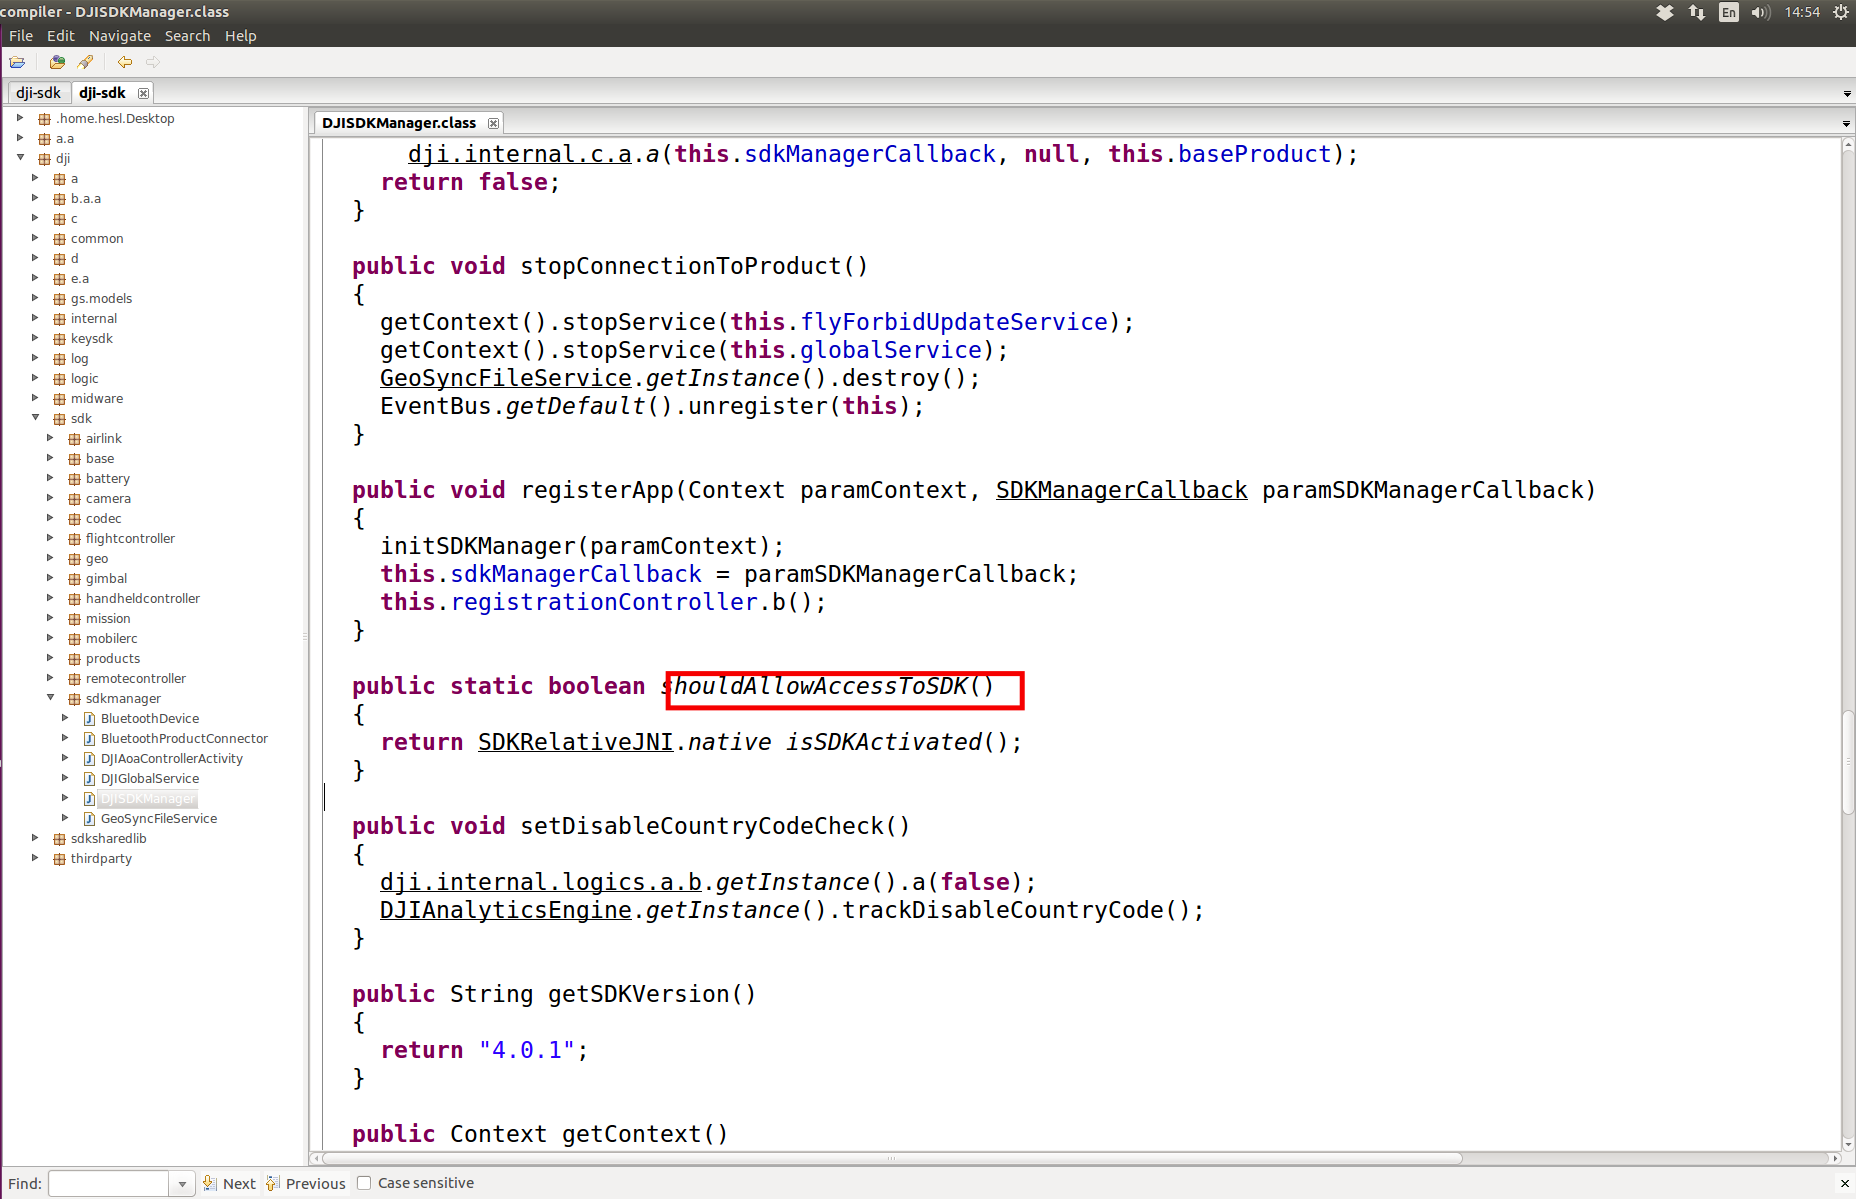
\includegraphics[width=0.9\columnwidth]{jd}
	\caption{Portion of decompiled SDKManager Class}
\end{figure} 
We decompiled the library jar file dji-sdk using \cite{jdgui} and edited the code using \cite{jbe}. We found functions registerApp, isSDKActivated,  shouldAllowAccessSDK, hasSDKRegistered mainly handling this authentication. startConnectionToProduct() which in turn calls shouldAllowAccessSDK(), checks whether the user will be given access to SDK, hasSDKRegistered() registered with a valid AppID(key) against a registered user, which is obtained after registration of an app. This key is pasted as AppID in the main Manifest.xml file of the customised app to activate DJI-SDK.\\
%\begin{figure}[h!]
%	\centering
%	\includegraphics[width=0.9\columnwidth]{jd1}
%	\caption{Patched code for shouldAllowAccessSDK}
%\end{figure}
We patched two functions shouldAllowAccessSDK(), hasSDKRegistered() to return true always without any further permission checking, thus effectively removing authentication. So even a wrong key or null string as AppID would not throw an error preventing opening of the app. This authentication is crucial to prevent any malicious user taking control over a drone of an authentic user. We built some custom apps for controlling camera, taking photos, videos and a playback manager using the cracked SDK. The custom apps showed successfull authentication, worked perfectly fine.
%screenshots

\subsubsection{Reverse engineering firmware}
The binary of the DJI Phantom 4 Pro firmware is encrypted and digitally signed. Though we were able to decrypt the binary, it was not possible to reflash with the new binary. The reason behind it probably being the binary not completely decrypted. We ran a customised parser and obtained two modules. Each of the module was first unpacked using rkflash\cite{rkflash}: a flashing tool for Rockchip based systems, and obtained standard images. In the Figure \ref{fig:reversing}, the image \emph{embedded-update.img} was further extracted into standard image modules: \emph{boot.img}, \emph{recovery.img}, \emph{system.img}. They were further unpacked into standard Android partitions using different Android image flash tools.
%\begin{figure}[h!]
%	\centering
%	\includegraphics[width=0.9\columnwidth]{rkunpack}
%	\caption{Standard Android partitions obtained}
%	\label{fig:reversing}
%\end{figure}
%screenshots

\subsubsection{GPS Spoofing}
DJI Phantom drones are GPS based drones; receiving incoming signals from GPS satellites, signals notifying the drone’s presence, and a two-way link between the ground station controller and the drone.
GPS enables a drone’s navigation, and due to no encryption of the civilian GPS signals they can be easily spoofed. The basic idea in GPS spoofing is transmitting fake GPS coordinates to the flight controller of the drone. This will hijack the drone and subsequently it will be in complete control of the attacker. To spoof a GPS receiver, a transmitter is used to transmit false GPS signals forcing the victim to synchronize with the attacker’s signals, including spoofed information regarding the ephemeris and almanac data. If the GPS receiver switches GPS fix from legitimate GPS signals to false GPS signals, drone deters its path and sends the drone in a direction specified by the attacker. A successful attack is conducted when attacker is very close to the drone, or by using a directional antenna of proper frequency aiming the drone.
\begin{figure}[h!]
	\centering
	\includegraphics[width=0.9\columnwidth]{images/setup}
	\caption{GPS Spoofing Setup}
	\label{fig:setup}
\end{figure}
\\
Though DJI improved the navigation by inertial measurement unit(IMU) instead of relying only on GPS. Still we managed to spoof the GPS receiver using LabSat3 GPS simulator\cite{labsat}. 
DJI Phantom 4 Pro comes with Ublox Neo 8M GPS receiver which has the ability to detect jamming with the help of J/N monitoring. J/N monitors triggers an alarm if the recieved power is more than the trigerring threshold, preventing jam-and-then-spoof kind of attack. We performed the spoofing attack inside a screened environment in the presence of weak real GPS signals. It was difficult to conduct the experiment outdoors due to the presence of strong legitimate GPS signals.
%%Explain our setup
\paragraph*{Experiment Procedure}
Here we perform record
and replay attack only. First real GPS signals are recorded using theactive antenna RLACS198 provided with the labsat kit. This antenna does not work as a transmitter.
For receiving signals, antenna is connected to SMA RF IN port.
Fake GPS signals can also be generated using SatGen software provided with LabSat. There is no tansmitter antenna provided with the kit. To replay, it needs a 1575 MHz (GPS L1 frequency) antenna for proper working and connected to RF OUT port.
\\
\begin{figure}[h!]
	\centering
	\includegraphics[width=0.9\columnwidth]{ntu}
	\caption{Initial location: NTU, Singapore}
	\label{fig:ntu}
\end{figure}
The location of the drone was successfully spoofed by LabSat. The drone was placed inside HESL lab at NTU. Though DJI Phantom 4 Pro has
ublox GPS module with J/N monitoring, it fails to detect spoofing in our case, as the transimitted power was very less. The location, altitude, speed is shown by the DJI Go 4 app.
Several kind of hacks are performed: force landing a drone spoofing the location to be a NFZ, flying a drone in a NFZ, height hack.
In the figure \ref{fig:ntu}, the drone is seen to be located at Nanyang Technological University, the spoofed location shows the drone to be in Changi South Avenue near SUTD in figure \ref{fig:nfz}, which is a no-fly-zone.
\begin{figure}[h!]
	\centering
	\includegraphics[width=0.9\columnwidth]{nfz}
	\caption{No Fly Zone near SUTD, Changi Airport}
	\label{fig:nfz}
\end{figure}
If it had been flying with real GPS, and we transmit fake GPS, and these are more stronger in quality than real ones and the spoofed location is a
NFZ, the drone would perform an emergency landing.
\\
Similarly the reverse experiment could be performed where the drone was located in a NFZ preventing the drone to take-off and if location is successfully spoofed to a non-restricted place, drone would take off.
\\
Also the movement of the drone could be faked by replaying any motion curve or pre-recorded data as in figure \ref{fig:drone mov} below.
\begin{figure}[h!]
	\centering
	\includegraphics[width=0.9\columnwidth]{moving}
	\caption{Drone Movement}
	\label{fig:drone mov}
\end{figure}
%screenshots

\subsection{Parrot Bebop 2}
Most of the attacks in Parrot Bebop 2 being tested are possible to the open WiFi. Even the Parrot manufacturers have introduced the feature of adding WPA/WPA2 password to the Bebop WiFi which obvioulsy decreases range and speed. Nonetheless, it remains vulnerable to WiFi attacks. Weak password can be easily cracked by tools like \cite{aircrack}.

\paragraph*{Network Mapping}
The nmap utility shows the ports used by the drone and the different services using it. By nmap scan of the drone's IP, we got 3 open ports running services ftp, telnet, tor-socks. 
%\begin{figure}[h!]
%	\centering
%	\includegraphics[width=0.9\columnwidth]{nmap_scan}
%	\caption{Nmap scan of IP: 192.168.42.1}
%	\label{fig:nmap}
%\end{figure}
%include picture

\subsubsection{Open WiFi}
Bebop 2 drone uses
an IEEE WiFi radio type of 802.11ac and the IP address of the drone is 192.168.42.1. 
An unencrypted open WiFi allows any one to connect and hijack the drone. Since Bebop2 allows for multiple clients to connect to the network, the problem is more critical i.e. more than one user can control the drone. There is no way of validating the original owner. 
\subsubsection{Deauthenticating owner}
We performed the deauthentication attack on the drone using \cite{aircrack}. This attack consists of capturing packets of the Bebop network without even connecting to it, diconnecting the authenticated owner. Initially the wireless network is scanned in monitor mode using airmon-ng. After the Bebop network is found, it snoops into the network using airodump-ng capturing all the packets from that network only. 
%\begin{figure}[h!]
%	\centering
%	\includegraphics[width=0.9\columnwidth]{deauth}
%	\caption{Deauthenticating the owner}
%	\label{fig: deauth}
%\end{figure}
When the list of clients are available, deauthentication attack is performed by executing aireplay-ng, which sends de-authentication packets continuously to the clients, disconnecting them until the program executes. In the meantime, the hacker gets connected and can hijack the drone being the only client connected.
\\
In the Figure \ref{fig: deauth}, deauthentication packets are send continuously from the attacker's laptop to the connected client whose MAC address is 48:88:CA:62:9B:A3 where the drone's BSSID is A0:14:3D:C1:F4:2B. The entire network can be jammed by sending disauthentication packets continuously, preventinf anyone to connect to the network. The aireplay-ng sends 128 deauth packets: 64 packets to BSSID and 64 packets to the client. In each last column of figure \ref{fig: deauth}, first number denotes the number of ACKs received from the client and second denotes that received from the drone.
\begin{figure}[h!]
	\centering
	\begin{subfigure}{.2\textwidth}
		\centering
		\includegraphics[width=0.85\columnwidth]{disconnec1}
		\caption{Owner Connected}
	\end{subfigure}$\xrightarrow[\text{Deauth.}]{\text{After}}$
	\begin{subfigure}{.2\textwidth}
		\centering
		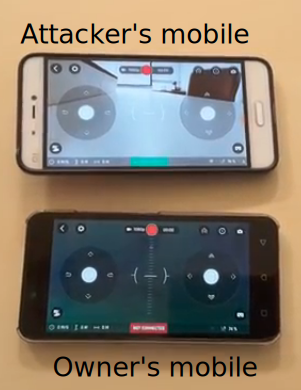
\includegraphics[width=0.85\columnwidth]{disconn2}
		\caption{Owner disconnected}
	\end{subfigure}
	\caption{Deauthenticating owner's mobile}
	\label{fig:disconnect}
\end{figure}
In the above Figure \ref{fig:disconnect}, the below mobile belonging to the owner remains disconnected as long as aireplay continues to send directed deauth packets. The attacker takes this advantage to connect his own mobile(above) and can hijack the drone.  

\subsubsection{Open Telnet}
Once connected to the Bebop 2 WiFi, the user can telnet to it. The drone's IP address is 192.168.42.1. Since multiple user can connect to the drone WiFi, just attempting to connect to the network, generates multiple requests in a short span of time, which may cause \textbf{DOS} attack, results in interrupting original commands. Even by telnetting to it, the user get root access to the entire file system. 
By telnetting into the drone, we were able to kill the main process \textit{dragon-prog},  which would stop motor arms immediately making the drone fall on the ground. \textit{dragon-­prog} is the main Bebop process governing the whole system of flight control.
We also found a list of other interesting processes running by \emph{ps} command of Unix. We also found important shell scripts
\emph{/usr/bin/ardrone3\_shutdown.sh}, \emph{/usr/bin/DragonStarter.sh}

We observed executing \emph{ardrone3\_shutdown.sh} also stopped the main process and the drone shuts down immediately. 

\subsubsection{Root access to file system}
Since the release of AR.Drone 3.0, most of the files are read-only, except the /data directory which is the FTP media directory. Though the files are by default read-only, the user can override it by remounting the entire file system by
\begin{lstlisting}[language =  bash]
# mount -o remount, rw /
\end{lstlisting}

%\begin{figure}[h!]
%	\centering
%	\includegraphics[width=0.9\columnwidth]{root_fs}
%	\caption{Root access to file system}
%	\label{fig:root_fs}
%\end{figure}
%list of interesting files


\subsubsection{Open FTP port}
Without any authentication for FTP, attackers may connect to the WiFi and login to the FTP to steal personal information including media, flight data, etc. Due to factory settings, FTP access does not allow to navigate the whole filesystem, but only the ftp directory \emph{/data/ftp/internal\_000}, which is where images and videos are recorded, together with other useful files like pud files.
The limited FTP access can be taken over by editing the file \emph{​/etc/inetd.conf}. ​
After the following lines, 
\begin{quote}
	21 stream tcp nowait root ftpd ftpd ­wSS /data/ftp
	\linebreak 
	51 stream tcp nowait root ftpd ftpd ­wSS /update
	\linebreak 
	61 stream tcp nowait root ftpd ftpd ­wSS	
\end{quote}
we need to add the following line to get access to entire file system:

\emph{71 stream tcp nowait root ftpd ftpd ­SS /} 

\subsubsection{Snooping into the WiFi and packet capture}
We used Wireshark to capture packets during the connection establishment and throughout the entire flight. The flight commands and video are passed as UDP packets while the initial connection setup is done by TCP. 

%include wireshark screenshots

\subsubsection{Additional vulnerabilties}
\paragraph{Reversing firmware}
The Bebop 2 firmware is completely reversible and can be easily modified and the new binary can be reflashed. Reversing firmware gives insight into the drone workflow and file system, which makes easier for the attacker to exploit vulnerabilities and target specific location.
\paragraph{Modifying files}
The entire file system can be accessed using telnet after being connected to the Bebop's WiFi. Wrong modification of configuration files/scripts like dragon.conf to crash the software and hamper normal operation of the drone. 
Modifying /etc/passwd file may brick the drone as changing some passwords may cause the owner not be able to telnet into it, or connect to the drone.

\section{Comparison of two drones}\label{Comparison of two drones}
From the different experiments conducted and keen observations made after analysis the security aspects of both the Phantom 4 Pro and Bebop 2 drones,
the comparison can be made on the basis of easiness to fly, image quality, processing speed, smoothness, security, etc. But the most significant of all is the security aspect of drones.
\\
It can be concluded that though Bebop 2 is more user-friendly, Phantom 4 Pro is more secure than Bebop 2. Phantom 4 Pro is only vulnerable to GPS spoofing and interception/jamming of radio signals using SDR. Bebop 2 is prone to different wireless attacks and can be easily hijacked. While SDR equipments and/or GPS spoofer are difficult to acquire in terms of availability and cost, several wireless tools and network scanner, analysers are readily available online free of cost. 
We also noticed that DJI tried to improve the security by introducing communication and video feed transmission via radio signals. DJI claims to have on-board FPGA video encryption algorithm which can be easily verified scanning transmitted radio signals using SDR or tapping the output of FPGA before it goes to the transceiver. DJI also encrypts the firmware partially and the binary is digitally signed, still it can be decrypted to some extent. 

\section{Proposed countermeasures}\label{Proposed countermeasures}
Below we propose some methods/actions that can be implemented to increase the security of drone. Drones shall remain vulnerable to GPS spoofing unless receiver also have the capability to detect spoofing like SAASM used by military- thus need for developing anti-spoofing and anti-jamming receivers. While there has been a lot of promising work and proposed methods in detection and avoidance of civilian GPS anti-spoofing and anti-jamming in the literature similar to that in \cite{wesson2012straight}. Those methods can be broadly classified into cryptographic: spread spectrum, dual receiver correlation and non-cryptographic methods: antenna array, requires external hardware. The above methoda are either difficult to implement or requires costly hardware. So we would like to propose simpler software based techniques for spoof detection:

\paragraph*{Checking latency}
The motion speed can be validated for the change in location in a short instant, for e.g. one cannot travel and change its location from new York to Beijing in few seconds. The changes of coordinates can be recorded and validated given the time taken to change the coordinates.
\paragraph*{Checking GPS subframe data}
\begin{figure}[h!]
	\centering
	\includegraphics[width=0.9\columnwidth]{gps}
	\label{fig:gps_frame}
	\caption{GPS subframes}
\end{figure}
The GPS frame starts with telemetry word used as preamble, which provides details of the satellite. Handover word(HOW) provides the GPS system time. HOW is followed by eight data words with parity bits. Subframe-1 carry information to correct the satellite clock. Subframe-2 and subframe-3 provides ephemeris data for the satellites. Subframe-4 and sunframe-5 send the Almanac data. 
GPS subframe data can be validated easily by checking each of the subframes. Fake GPS data is observed to have wrong subframe data, thus able to detect spoofing. 
Thus an onboard Raspberry Pi on the drone validating time-motion or GPS subframe data can easily detect gps spoofing.
\\
Apart from GPS anti-spoofing and anti-jamming, we would like to recommend some modifications which can improve the security of drone. 
\begin{itemize}
	\item Using encryption/packer to protect library files
	\item Using obfuscator to prevent decompiling, reverse-engineering files
	\item Improve SDK authentication, now being done only between the app and server, drone must also be included in the one-time authentication
	\item Encrypt the entire firmware binary, the encryption key must be stored in the hardware
\end{itemize}

On the contrary, many of the attacks described above for Bebop 2 are possible only due to open WiFi and open ports. Additionally FTP need not be activated inflight to prevent stealing of flight data and media. This is enough to secure personal data if after flight this data can be backed up offline. For Bebop 2, generally WiFi-based UAVs, we propose the following countermeasures:
\paragraph{Adding WPA security}
With the release of ARDrone3, Parrot developers introduced the feature of adding WPA/WPA2 security to the WiFi using Freeflight Pro app. Nonetheless with powerful WiFi password cracking tools like aircrack-ng, it is possible to crack the password. Also augmenting security causes decrease in range and transmission speed. 
\paragraph{Adding telnet password}
Bebop 2 should not allow root access to the file system once connected and telnetted. This can be managed by adding a telnet password modifying \emph{/etc/passwd} file. 
\paragraph{MAC-filtering and Hidden SSID}
These can be achieved through bcmwl program installed in the drone. bcmwl controls all the wireless wi-fi connectivity of the drone. Any changes made can be temporary or permanent. In order to reversibly hide the wifi SSID, open a telnet session and enter the following command:

\begin{lstlisting}
  # bcmwl closed 1
\end{lstlisting} 

This makes it more difficult for others to connect to the drone, since the wifi network will not appear in the list of available networks.

To activate MAC address filtering, 
\begin{lstlisting}
  # bcmwl mac MA:CA:DD:RE:SS:01 MA:CA:DD:
  RE:SS:02 ...
\end{lstlisting} 
where all the possible MAC addresses are given by the owner followed by:
\begin{lstlisting}
  # bcmwl macmode 2
\end{lstlisting} 

which sets MAC filtering to only accept connections from the previous list of devices. To permanently introduce these changes, we need to modify
\emph{/sbin/broadcom\_setup.sh} file.
% An example of a floating figure using the graphicx package.
% Note that \label must occur AFTER (or within) \caption.
% For figures, \caption should occur after the \includegraphics.
% Note that IEEEtran v1.7 and later has special internal code that
% is designed to preserve the operation of \label within \caption
% even when the captionsoff option is in effect. However, because
% of issues like this, it may be the safest practice to put all your
% \label just after \caption rather than within \caption{}.
%
% Reminder: the "draftcls" or "draftclsnofoot", not "draft", class
% option should be used if it is desired that the figures are to be
% displayed while in draft mode.
%
%\begin{figure}[!t]
%\centering
%\includegraphics[width=2.5in]{myfigure}
% where an .eps filename suffix will be assumed under latex, 
% and a .pdf suffix will be assumed for pdflatex; or what has been declared
% via \DeclareGraphicsExtensions.
%\caption{Simulation results for the network.}
%\label{fig_sim}
%\end{figure}

% Note that the IEEE typically puts floats only at the top, even when this
% results in a large percentage of a column being occupied by floats.


% An example of a double column floating figure using two subfigures.
% (The subfig.sty package must be loaded for this to work.)
% The subfigure \label commands are set within each subfloat command,
% and the \label for the overall figure must come after \caption.
% \hfil is used as a separator to get equal spacing.
% Watch out that the combined width of all the subfigures on a 
% line do not exceed the text width or a line break will occur.
%
%\begin{figure*}[!t]
%\centering
%\subfloat[Case I]{\includegraphics[width=2.5in]{box}%
%\label{fig_first_case}}
%\hfil
%\subfloat[Case II]{\includegraphics[width=2.5in]{box}%
%\label{fig_second_case}}
%\caption{Simulation results for the network.}
%\label{fig_sim}
%\end{figure*}
%
% Note that often IEEE papers with subfigures do not employ subfigure
% captions (using the optional argument to \subfloat[]), but instead will
% reference/describe all of them (a), (b), etc., within the main caption.
% Be aware that for subfig.sty to generate the (a), (b), etc., subfigure
% labels, the optional argument to \subfloat must be present. If a
% subcaption is not desired, just leave its contents blank,
% e.g., \subfloat[].


% An example of a floating table. Note that, for IEEE style tables, the
% \caption command should come BEFORE the table and, given that table
% captions serve much like titles, are usually capitalized except for words
% such as a, an, and, as, at, but, by, for, in, nor, of, on, or, the, to
% and up, which are usually not capitalized unless they are the first or
% last word of the caption. Table text will default to \footnotesize as
% the IEEE normally uses this smaller font for tables.
% The \label must come after \caption as always.
%
%\begin{table}[!t]
%% increase table row spacing, adjust to taste
%\renewcommand{\arraystretch}{1.3}
% if using array.sty, it might be a good idea to tweak the value of
% \extrarowheight as needed to properly center the text within the cells
%\caption{An Example of a Table}
%\label{table_example}
%\centering
%% Some packages, such as MDW tools, offer better commands for making tables
%% than the plain LaTeX2e tabular which is used here.
%\begin{tabular}{|c||c|}
%\hline
%One & Two\\
%\hline
%Three & Four\\
%\hline
%\end{tabular}
%\end{table}


% Note that the IEEE does not put floats in the very first column
% - or typically anywhere on the first page for that matter. Also,
% in-text middle ("here") positioning is typically not used, but it
% is allowed and encouraged for Computer Society conferences (but
% not Computer Society journals). Most IEEE journals/conferences use
% top floats exclusively. 
% Note that, LaTeX2e, unlike IEEE journals/conferences, places
% footnotes above bottom floats. This can be corrected via the
% \fnbelowfloat command of the stfloats package.




\section{Future Work and Conclusion}
We had to leave some portion as future work due to unavailability of proper hardware.  
We did not yet scan the radio signals through which the P4P communicates. It can be scanned and analysed using SDR equipments like HackRF, BladeRF. As further work, the transmission of video and control commands using packet style can be studied which DJI claims that it uses frequency hopping spread spectrum(FHSS). Though DJI manufacturers claim that the live video feed transmitted is encrypted using on-board FPGA encryption algorithm, it is yet to be verified. 
As further work for the Bebop 2 drone, we look forward to build Arducopter- an autonomous flight controller on top of it. \\
In conclusion, the P4P is one of the most secure and robust drones in the commercial market. Though DJI has developed P4P such that it is less vulnerable than its preedecessors, still it needs further work and a security analysis is worthwhile. Whereas Parrot manufacturers did not employ any security mesure for Bebop drones, Bebop 2 is too risky for any personal or commercial use. We believe the recommendations proposed as countermeasures would improve the security of Bebop drone and make it suitable for nominal use.\\
Future smart cities will be swarming with drones for different commercial and personal purposes in the hope that it will improve the lives of human being. 
With increasing reliability and dependency on technology, vulnerability becomes prominent and security becomes a chief concern. Drone manufacturers must employ techniques to improve the drone security, make it robust to attacks. Even if the drone can not be made entirely fool-proof, it must be resistant to easy wireless hacks and signal jamming or interception. \\
% conference papers do not normally have an appendix


% use section* for acknowledgment
\section*{Acknowledgment}


The authors would like to thank...





% trigger a \newpage just before the given reference
% number - used to balance the columns on the last page
% adjust value as needed - may need to be readjusted if
% the document is modified later
%\IEEEtriggeratref{8}
% The "triggered" command can be changed if desired:
%\IEEEtriggercmd{\enlargethispage{-5in}}

% references section

% can use a bibliography generated by BibTeX as a .bbl file
% BibTeX documentation can be easily obtained at:
% http://mirror.ctan.org/biblio/bibtex/contrib/doc/
% The IEEEtran BibTeX style support page is at:
% http://www.michaelshell.org/tex/ieeetran/bibtex/
%\bibliographystyle{IEEEtran}
% argument is your BibTeX string definitions and bibliography database(s)
%\bibliography{IEEEabrv,../bib/paper}
%
% <OR> manually copy in the resultant .bbl file
% set second argument of \begin to the number of references
% (used to reserve space for the reference number labels box)
\bibliographystyle{unsrt}
\bibliography{ref_drone}





% that's all folks
\end{document}


